\documentclass[11pt]{article}
\usepackage{graphicx}
\usepackage{amssymb}
\usepackage{amssymb}
\usepackage{latexsym, amsmath, amscd,amsthm}
\usepackage{graphicx}
\usepackage[percent]{overpic}
\usepackage{pdfsync}
\usepackage{units}
\usepackage{epstopdf}
\usepackage{pdfpages}
\usepackage{listings}

\usepackage{paralist}
\usepackage{color}

\usepackage{forest}

\DeclareGraphicsRule{.tif}{png}{.png}{`convert #1 `dirname #1`/`basename #1 .tif`.png}

%\addtolength{\textwidth}{90pt}
%\addtolength{\evensidemargin}{-60pt}
%\addtolength{\oddsidemargin}{-60pt}
%\addtolength{\topmargin}{-100pt}
%\addtolength{\textheight}{2in}

	\addtolength{\oddsidemargin}{-.875in}
	\addtolength{\evensidemargin}{-.875in}
	\addtolength{\textwidth}{1.75in}

	\addtolength{\topmargin}{-1in}
	\addtolength{\textheight}{2in}

%%%%%%%%%%%%%%%%%%%%%%%%%%%%%%%%%%%%%%%%%%%%%%
% For including sections of code

\usepackage{fancyvrb}
\DefineVerbatimEnvironment{code}{Verbatim}{fontsize=\small}


%%%%%%%%%%%%%%%%%%%%%%%%%%%%%%%%%%%%%%%%%%%%%%
%  Begin user defined commands

\newcommand{\map}[1]{\xrightarrow{#1}}

\newcommand{\C}{\mathbb C}
\newcommand{\F}{\mathbb F}
%\newcommand{\H}{\mathbb H}
%\newcommand{\N}{\mathbb N}
\newcommand{\Z}{\mathbb Z}
\newcommand{\Prob}{\mathbb{P}}
\newcommand{\Q}{\mathbb Q}
\newcommand{\R}{\mathbb R}


\newcommand{\zbar}{\overline{\mathbb{Z}}}
\newcommand{\qbar}{\overline{\mathbb{Q}}}

\newcommand{\la}{\langle}
\newcommand{\ra}{\rangle}
\newcommand{\lra}{\longrightarrow}
\newcommand{\hra}{\hookrightarrow}
\newcommand{\bs}{\backslash}

\newcommand{\al}{\alpha}
\newcommand{\be}{\beta}

%%stats commands
\newcommand{\E}{\mathrm{E}}
\newcommand{\Var}{\mathrm{Var}}
\newcommand{\Cov}{\mathrm{Cov}}

%%% Text Commands
\newcommand{\tand}{\text{ and }}
\newcommand{\tfor}{\text{ for }}
\newcommand{\ton}{\text{ on }}
\newcommand{\tin}{\text{ in }}
\newcommand{\tif}{\text{ if }}

\newcommand{\vectornorm}[1]{\left|\left|#1\right|\right|}

\DeclareMathOperator{\Aut}{Aut}
\DeclareMathOperator{\Aff}{Aff}
\DeclareMathOperator{\End}{End}
\DeclareMathOperator{\Hom}{Hom}
\DeclareMathOperator{\im}{im}

%  End user defined commands
%%%%%%%%%%%%%%%%%%%%%%%%%%%%%%%%%%%%%%%%%%%%%%


%%%%%%%%%%%%%%%%%%%%%%%%%%%%%%%%%%%%%%%%%%%%%%
% These establish different environments for stating Theorems, Lemmas, Remarks, etc.

\newtheorem{Thm}{Theorem}
\newtheorem{Prop}[Thm]{Proposition}
\newtheorem{Lem}[Thm]{Lemma}
\newtheorem{Cor}[Thm]{Corollary}

\theoremstyle{definition}
\newtheorem{Def}[Thm]{Definition}

\theoremstyle{remark}
\newtheorem{Rem}[Thm]{Remark}
\newtheorem{Ex}[Thm]{Example}

\theoremstyle{definition}
\newtheorem{Problem}{Problem}

\newenvironment{Solution}{\noindent{\it Solution.}}{\qed}

\tikzset{
Above/.style={
  midway,
  above,
  font=\scriptsize,
  text width=3.8cm,
  align=center,
  },
Below/.style={
  midway,
  below,
  font=\scriptsize,
  text width=3.8cm,
  align=center
  }
}


% End environments 
%%%%%%%%%%%%%%%%%%%%%%%%%%%%%%%%%%%%%%%%%%%%%%%


\begin{document}

\author{Betsy Cowdery}
\title{Bayesian Statistics HW 1}
\date{}
\maketitle

\begin{enumerate}

\item BDA 1.1 \\ Conditional probability: suppose that if $\theta = 1$, then y has a normal distribution with mean 1 and standard deviation $\sigma$, and if $\theta = 2$, then y has a normal distribution with mean 2 and standard deviation $\sigma$. Also, suppose $P(\theta = 1) = 0.5$ and $P(\theta = 2) = 0.5$

\begin{enumerate}
\item For $\sigma = 2$, write the formula for the marginal probability density for y and sketch it.

\begin{align*}
	P(y) 
&= \sum_{\tilde{\theta} \in \{\theta_1, \theta_2\}} P(y,\tilde{\theta}) P(\tilde\theta)\\
&= P(y,\theta_1)P(\theta_1)+P(y,\theta_2)P(\theta_2)\\
&= N(1,2)(.5)+N(2,2)(.5)
\end{align*}

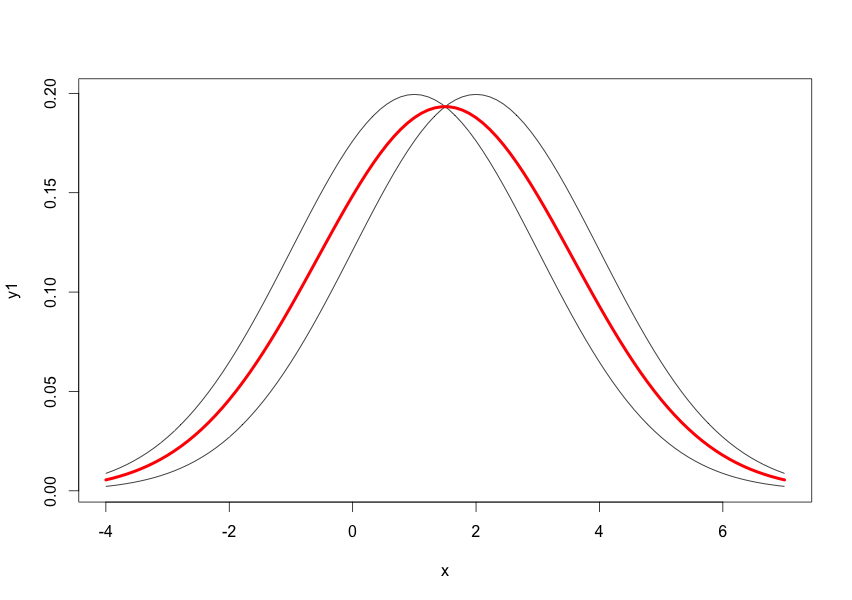
\includegraphics[scale=.4]{dist_1}


\item What is $Pr(\theta = 1|y = 1)$, again supposing $\sigma = 2$?

\begin{align*}
	P(\theta = 1|y = 1) 
	&= P(y=1|\theta=1)P(\theta=1)/P(y=1)\\
	&= .19*.5/.2 \\
	&\approx .47
\end{align*}
 

\newpage
\item Describe how the posterior density of $\theta$ changes in shape as $\sigma$ is increased and as it is decreased.

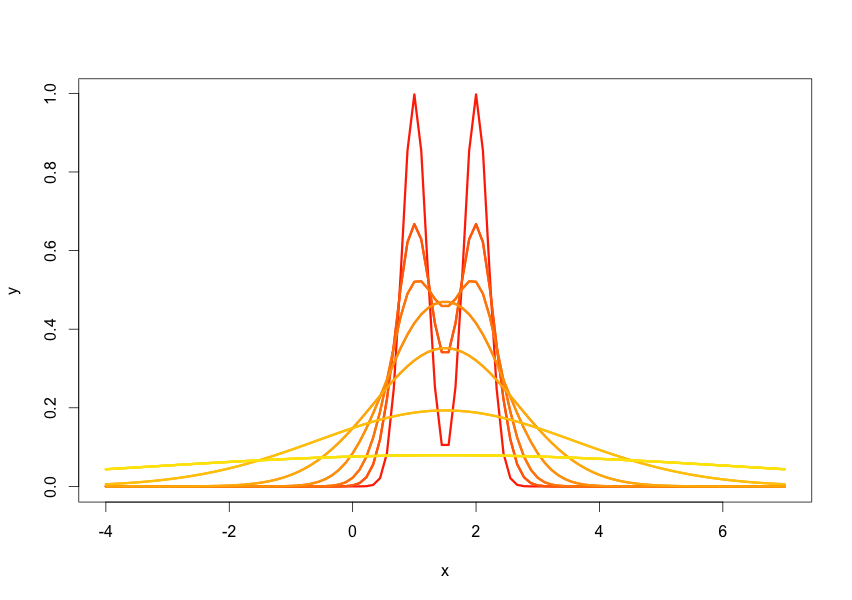
\includegraphics[scale=.4]{dist_2}

\end{enumerate}


\item BDA 1.3\\ Probability calculation for genetics (from Lindley, 1965): suppose that in each individual of a large population there is a pair of genes, each of which can be either x or X, that controls eye color: those with xx have blue eyes, while heterozygotes (those with Xx or xX) and those with XX have brown eyes. The proportion of blue-eyed individuals is $p^2$ and of heterozygotes is $2p(1 - p)$, where $0 < p < 1$. Each parent transmits one of its own genes to the child; if a parent is a heterozygote, the probability that it transmits the gene of type X is $1/2$. 

\begin{forest} 
for tree={
  grow=east,
  draw=cyan,
  reversed=true,
  line width=0.2pt,
  parent anchor=east,
  child anchor=west,
  edge={draw=cyan},
  edge label={\Huge\color{black}},
  edge path={
    \noexpand\path[\forestoption{edge}]
      (!u.parent anchor) -- ([xshift=-3.1cm].child anchor) --    
      (.child anchor)\forestoption{edge label};
  },
  l sep=3.3cm,
  s sep=(4-level)*.3cm
} 
[, rectangle, 
  [,edge label={node[Above]{$P(H) = 2p(1-p)$}}
    [,edge label={node[Above]{$P(B|H) = 1$}}
	    [{$P(X,B,H) = p(1-p)$},edge label={node[Above]{$P(X|B,H) = 1/2$}}]
    	[{$P(x,B,H) = p(1-p)$},edge label={node[Below]{$P(x|B,H) = 1/2$}}]
    ]
%    [,edge label={node[Below]{$P(NB|H) = 0$}}]
   ]
   [,edge label={node[Below]{$P(NH) = 1-2p(1-p)$}}
   	[,edge label={node[Above]{$P(B|NH) = \frac{(p-1)^2}{1-2p+2p^2}$}}
    	[{$P(X,B,NH) = (p-1)^2$},edge label={node[Above]{$P(X|B,NH) = 1$}}]
%    	[,edge label={node[Below]{$P(x|B,NH) = 0$}}]
    ]
    [,edge label={node[Below]{$P(NB|NH) = \frac{p^2}{1-2p+2p^2}$}}
%    	[,edge label={node[Above]{$P(X|NB,NH) = 0$}}]
    	[{$P(x, NB, NH) = p^2$},edge label={node[Below]{$P(x|NB,NH) = 1$}}] 
    ]
  ]
]
\end{forest}

Assuming random mating, show that among brown-eyed children of brown-eyed parents, the expected proportion of heterozygotes is $2p/(1 + 2p)$. \\


Suppose Judy, a brown-eyed child of brown-eyed parents, marries a heterozygote, and they have n children, all brown-eyed. Find the posterior probability that Judy is a heterozygote and the probability that her first grandchild has blue eyes.




\newpage
\item Simpson’s paradox\\ In a medical study to determine the effectiveness of two different treatments, A and B, for two different types of kidney stones, “small” and “large”, the researchers found the following success rates: for treatment A, 93\% success on small stone cases and 73\% success on large stone cases; for treatment B, 87\% success on small stone cases and 69\% success on large stone cases. It is assumed that 51\% of kidney stone cases are due to small stones
\begin{enumerate}
\item The experimental design of the study assigned 24\% of small stone cases to treatment A and 77\% of large stone cases to treatment A. If a patient is selected at random from treatment A, what is the probability that she has small stones? What is the probability of her having small stones given that she was now selected from treatment B?\\


\begin{forest} 
for tree={
  grow=east,
  draw=cyan,
  reversed=true,
  line width=0.2pt,
  parent anchor=east,
  child anchor=west,
  edge={draw=cyan},
  edge label={\color{black}},
  edge path={
    \noexpand\path[\forestoption{edge}]
      (!u.parent anchor) -- ([xshift=-3.1cm].child anchor) --    
      (.child anchor)\forestoption{edge label};
  },
  l sep=3.3cm,
  s sep=(4-level)*.2cm
} 
[, rectangle, 
  [,edge label={node[Above]{$P(s) = 0.51$}}
    [,edge label={node[Above]{$P(A|s) = 0.24$}}
	    [{$P(s,A,S) \approx 0.1138$},edge label={node[Above]{$P(S|A,s) = 0.93$}}]
    	[{$P(s,A,F) \approx 0.0086$},edge label={node[Above]{$P(F|A,s) = 0.70$}}]
    ]
    [,edge label={node[Above]{$P(B|s) = 0.76$}}
	    [{$P(s,B,S) \approx 0.3372$},edge label={node[Above]{$P(S|B,s) = 0.87$}}]
    	[{$P(s,B,F) \approx 0.0504$},edge label={node[Above]{$P(F|B,s) = 0.13$}}]
    ]
  ]
  [,edge label={node[Above]{$P(l) = 0.49$}}
    [,edge label={node[Above]{$P(A|l) = 0.77$}}
	    [{$P(l,A,S) \approx 0.2754$},edge label={node[Above]{$P(S|A,l) = 0.73$}}]
    	[{$P(l,A,F) \approx 0.1019$},edge label={node[Above]{$P(F|A,l) = 0.27$}}]
    ]
    [,edge label={node[Above]{$P(B|l) = .23$}}
	    [{$P(l,B,S) \approx 0.0778$},edge label={node[Above]{$P(S|B,l) = 0.69$}}]
    	[{$P(l,B,F) \approx 0.0349$},edge label={node[Above]{$P(F|B,l) = 0.31$}}]
    ]
  ]
]
\end{forest}\\

$$P(s|A) = \frac{P(A|s)P(s)}{P(A)} = \frac{(.24)*(.51)}{(.24)*(.51) + (.77)(.49)} \approx .245$$
$$P(s|B) = \frac{P(B|s)P(s)}{P(B)} = \frac{(.76)*(.51)}{(.76)*(.51) + (.23)(.49)} \approx .775$$



\item What are the (marginal) success rates of treatments A and  B? How do they compare to the (conditional) success rates given the conditions small and large stones? How would you explain the discrepancies in light of the probabilities computed in (a)?

$$P(S|A) = \frac{P(A,S)}{P(A)} = \frac{P(s,A,S) + P(l,A,S)}{P(A|s)P(s) + P(A|l)P(l)} \approx .779$$
$$P(B,S) = \frac{P(B,S)}{P(B)} = \frac{P(s,B,S) + P(l,B,S)}{P(B|s)P(s) + P(B|l)P(l)} \approx .830$$
So from this perspective, it appears that treatment B is better. \\
But the conditional success rates tell another story. 
$$P(S|A,s) = 0.93 \tand P(S|A,l) = 0.73$$
$$P(S|B,s) = 0.87 \tand P(S|B,l) = 0.69$$
Here it appears that treatment A is better. \\

\item The discrepancy above is known as “Simpson’s paradox”, and in this case seems to stem from the poor experimental design. Let us investigate this further: call pAS and pAL the probabilities of a small stone case and a large stone case, respectively, being assigned to treatment A. Plot a heatmap of the ratio $\rho$ of success rates between treatments A and B as a function of pAS and pAL, and identify the region with $\rho < 1$, that is, where we see a paradox. Explain any patterns you see in the region, e.g., when pAS $>$ pAL.(Can you identify the isolines for $\rho$? If possible, try to show that they are hyperbolae, and for a specific value of $\rho$ a parabola! )

\begin{align*}
\rho 
&= \frac{P(S|A)}{P(S|B)} \\
&= \frac{P(s,A,S) + P(l,A,S)}{ P(s,B,S) + P(l,B,S)} * \frac{P(B)}{P(A)} \\
&= \frac{P(s)*pAS*P(S|A,s)) + P(l)*pAL*P(S|A,l))}{P(s)*(1-pAS)*P(S|B,s)) + P(l)*(1-pAL)*P(S|B,l))} * 
	\frac{(1-pAS)P(s) + (1-pAL)P(l)}{pAS*P(s) + pAL*P(l)}
\end{align*}

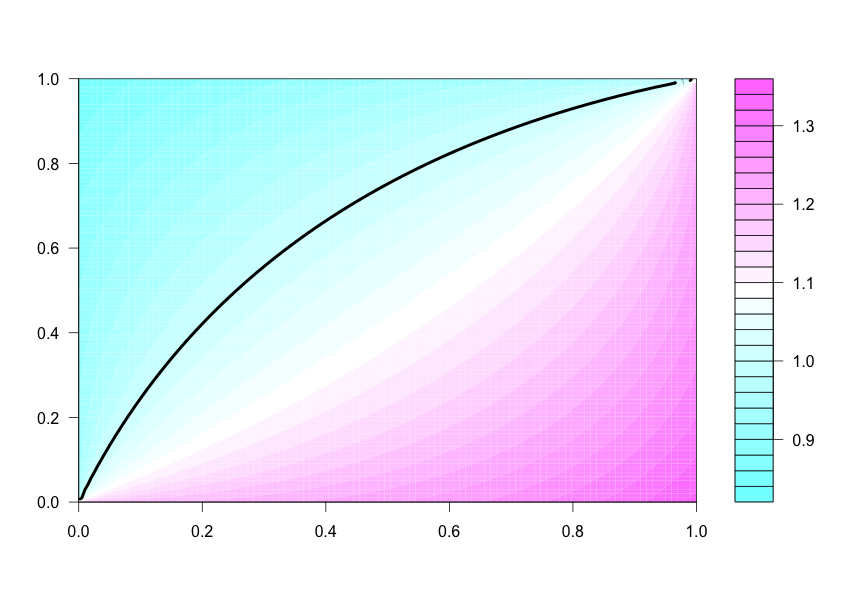
\includegraphics[scale=.4]{heat}



\end{enumerate}
\end{enumerate}
\end{document}